%
% Tutorial -- 10dB Directional Coupler Design
%
% Copyright (C) 2005 Stefan Jahn <stefan@lkcc.org>
%
% Permission is granted to copy, distribute and/or modify this document
% under the terms of the GNU Free Documentation License, Version 1.1
% or any later version published by the Free Software Foundation.
%

\tutsection{10dB Directional Coupler Design}

The below pictures shows two parallel conductor strips on a dielectric
substrate with a backplane metalization.  Both the conductor strips
have the width $W$, the height $t$ and the length $l$.  There is a
finite gap $S$ between the conductors.  The substrates height is
denoted by $h$.  With the gap between the conductor strips small
enough a capacitive as well as inductive coupling occurs.

\begin{figure}[ht]
  \centering
  \includegraphics[width=0.7\linewidth]{mcoupled}
  \caption{microstrip directional coupler}
  \label{fig:mcoupled}
\end{figure}
\FloatBarrier

Such a microstrip structure is called ``microstrip coupled lines''.
Also defined in figure \ref{fig:mcoupled} the port numbers 1\ldots 4.

\tutsubsection{Some boring theory beforehand}

There are two types of directional couplers: backward (coupling from
port 1 to port 4) and forward (coupling from port 1 to port 3)
couplers.

\addvspace{12pt}

The S-parameters of an ideal directional backward coupler are as
follows -- with $C$ denoting the coupling coefficient.
\begin{align*}
S_{21} &= \sqrt{1 - C^2}\\
S_{41} &= C\\
S_{31} &= 0\\
S_{11} = S_{22} = S_{33} = S_{44} &= 0
\end{align*}

In a three conductor system -- as the microstrip coupled lines are --
there are two types of modes: even and odd.  Thus such a system is
described by odd and even characteristic impedances ($Z_{L,o}$ and
$Z_{L,e}$) and odd and even effective dielectric constants
($\varepsilon_{r,eff,o}$ and $\varepsilon_{r,eff,e}$).  The
characteristic equations for an ideal backward coupler are
\begin{align*}
\varepsilon_{r,eff,e} &= \varepsilon_{r,eff,o}\\
Z_{L,e} &\ne Z_{L,o}
\end{align*}
and those for an ideal forward coupler are
\begin{align*}
\varepsilon_{r,eff,e} &\ne \varepsilon_{r,eff,o}\\
Z_{L,e} &= Z_{L,o}
\end{align*}

The S-parameters of the ideal directional forward coupler are as
follows.
\begin{align*}
S_{21} &= \sqrt{1 - C^2}\\
S_{31} &= C\\
S_{41} &= 0\\
S_{11} = S_{22} = S_{33} = S_{44} &= 0
\end{align*}

For both ideal -- forward and backward -- couplers the reflection
coefficients are zero.  Port 1 is called the \textbf{injection port}.
Port 2 is the \textbf{transmission port}.  In a backward coupler port
4 is the \textbf{coupled port} and port 3 is called the
\textbf{isolated port}.  In a forward coupler it's the other way
around.

\addvspace{12pt}

\textit{Please note:} The given S-parameters for forward and backward
couplers are valid for all side termination of each port with the
reference impedance $Z_L$ -- usually $50\ohm$.

\tutsubsection{Design equations}

In microwave labs backward line couplers are most wide spread.  The
basic design equations can be written as
\begin{align*}
C &= \dfrac{Z_{L,e} - Z_{L,o}}{Z_{L,e} + Z_{L,o}}\\
\beta\cdot l &= \dfrac{\pi}{2}\\
Z_L^2 &= Z_{L,o}\cdot Z_{L,e}\\
Z_{L,e} &= Z_L\cdot\sqrt{\dfrac{1 + C}{1 - C}}\\
Z_{L,o} &= Z_L\cdot\sqrt{\dfrac{1 - C}{1 + C}}
\end{align*}
With
\begin{align*}
\beta\cdot l &= \dfrac{\pi}{2}\\
\leadsto l &= \dfrac{\pi}{2\cdot \beta} = \dfrac{\pi\cdot c}{2\cdot \omega} = \dfrac{c}{4\cdot f} = \dfrac{\lambda}{4}
\end{align*}
the length $l$ of such a coupler is defined by a quarter wavelength.
Both the characteristic impedances can be computed by the reference
impedance $Z_L$, i.e. $50\ohm$, and the coupling coefficient $C$.

\tutsubsection{Applying the design equations}

With the previous definitions it's easy to design the 10dB directional
backward coupler.  We have the reference impedance $Z_L = 50\ohm$ and
the coupling coefficient $C$ in dB.  First we linearize the coupling
coefficient.
\begin{align*}
C_{dB} &= -10\textrm{dB}\\
\leadsto C &= 10^{C_{dB} / 20} = 10^{-0.5} \approx 0.316
\end{align*}
Now we compute the even and odd impedances.
\begin{align*}
Z_{L,e} &= Z_L\cdot\sqrt{\dfrac{1 + C}{1 - C}} \approx 69.4\ohm\\
Z_{L,o} &= Z_L\cdot\sqrt{\dfrac{1 - C}{1 + C}} \approx 36.0\ohm
\end{align*}

\tutsubsection{What next?}

All grey theory you may think...  With the impedances at hand the
engineer had to go into magic diagrams and find physical dimensions of
his coupler.  But now there is Qucs.  Things get easier.

\addvspace{12pt}

Just select \textbf{Tools} $\rightarrow$ \textbf{Line Calculation} in
the menubar or press \textbf{Ctrl+3} to start the transmission line
calculator.

\addvspace{12pt}

Then choose \textbf{Coupled Microstrip} in the \textbf{Transmission
Line Type} selection box.  Something likely shown in figure
\ref{fig:trcalc} should appear.

\begin{figure}[ht]
  \centering
  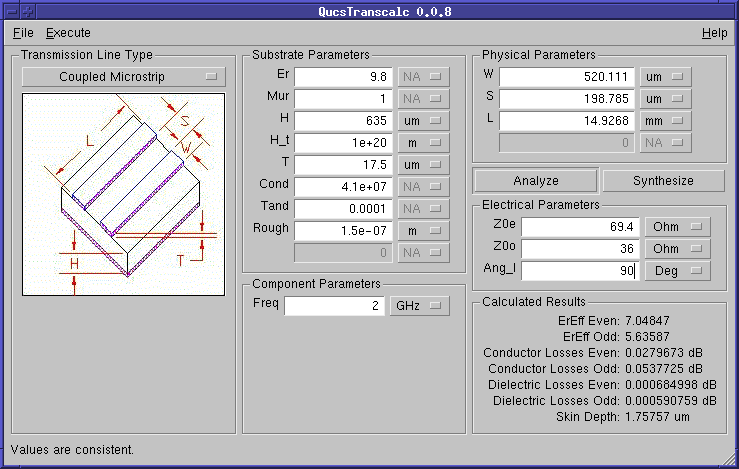
\includegraphics[width=1\linewidth]{coupledtrcalc}
  \caption{Qucs Transcalc screenshot}
  \label{fig:trcalc}
\end{figure}
\FloatBarrier

Type in the calculated \textbf{69.4} in the \textbf{Z0e} field,
\textbf{36.0} in the \textbf{Z0o} field and \textbf{90} in the
\textbf{Ang\_l} field of the \textbf{Electrical Parameters} panel.
The \textbf{Ang\_l} field denotes the desired electrical length of the
line (remember: $90\degree \simeq \pi/2$).  Choose the \textbf{Deg}
unit.

\addvspace{12pt}

Our selected design frequency is $2\giga\hertz$.  Thus type in this
value in the \textbf{Freq} field of the \textbf{Component Parameters}
panel.

\addvspace{12pt}

Then press the \textbf{Synthesize} button or press \textbf{F4}.  The
program calculates the physical parameters \textbf{W}, \textbf{S} and
\textbf{L} in the \textbf{Physical Parameters} panel.

\addvspace{12pt}

\textit{Please note:} Depending on the substrate (shown in the
\textbf{Substrate Parameters} panel) the calculated values may vary.

\addvspace{12pt}

Finally we got
\begin{align*}
W &= 520 \micro\meter\\
S &= 199 \micro\meter\\
L &= 14.93 \milli\meter
\end{align*}
All done with designing...  Feel any better?

\tutsubsection{Verification of the design}

Ok.  Let's verify what we have designed so far.  Choose
\textbf{Execute} $\rightarrow$ \textbf{Copy to Clipboard} from the
menubar or press \textbf{F2}.  This copies the currently shown
microstrip coupled line in Qucs Transcalc into the global clipboard.

\addvspace{12pt}

Now switch to an empty Qucs schematic and press \textbf{Ctrl+V}.  This
inserts the previously entered clipboard content -- and click with the
left mouse button in order to place the selection into the schematic.
This should give you something likely shown in figure
\ref{fig:coupledsch}.

\begin{figure}[ht]
  \centering
  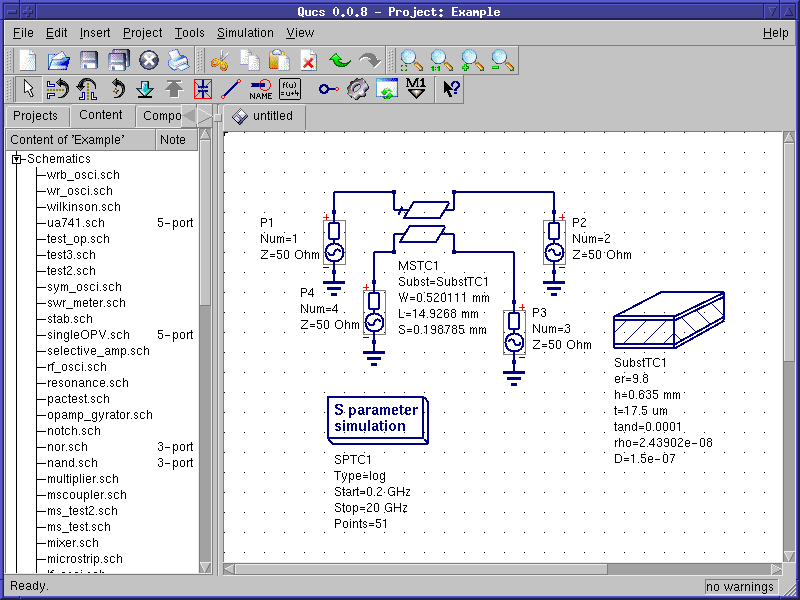
\includegraphics[width=1\linewidth]{coupledsch}
  \caption{coupled microstrip lines in a Qucs schematic}
  \label{fig:coupledsch}
\end{figure}
\FloatBarrier

Now press the equation button (shown in figure \ref{fig:eqnbutton}) in
Qucs's toolbar.

\begin{figure}[ht]
  \centering
  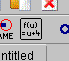
\includegraphics[width=0.2\linewidth]{eqnbutton}
  \caption{equation button}
  \label{fig:eqnbutton}
\end{figure}
\FloatBarrier

Place the equation into the schematic and enter the following
equations.  Press \textbf{Add} in the equation dialog (see figure
\ref{fig:eqndialog}) to add new equations.  Finally press the
\textbf{OK} button.

\begin{figure}[ht]
  \centering
  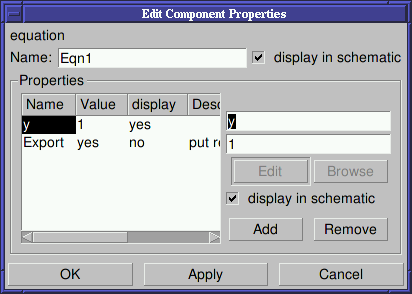
\includegraphics[width=0.6\linewidth]{eqndialog}
  \caption{equation dialog}
  \label{fig:eqndialog}
\end{figure}
\FloatBarrier

Also edit the properties of the \textbf{MSTC1} component reducing the
number of digits.  This will ensure that your technology is able to
use these values when (if) they decide to produce your design.

\addvspace{12pt}

Now edit the S-parameter simulation properties.  You can do that
either by double clicking the component and use the component dialog.
Or you can directly click on the values in the schematic and fill in
\textbf{0.2 GHz} for \textbf{Start}, \textbf{4.2 GHz} for
\textbf{Stop} and \textbf{101} for \textbf{Points}.

\addvspace{12pt}

Finally save your schematic by pressing \textbf{Ctrl+S}.  Check
whether all looks like as shown in figure \ref{fig:mscouplersch}.

\begin{figure}[ht]
  \centering
  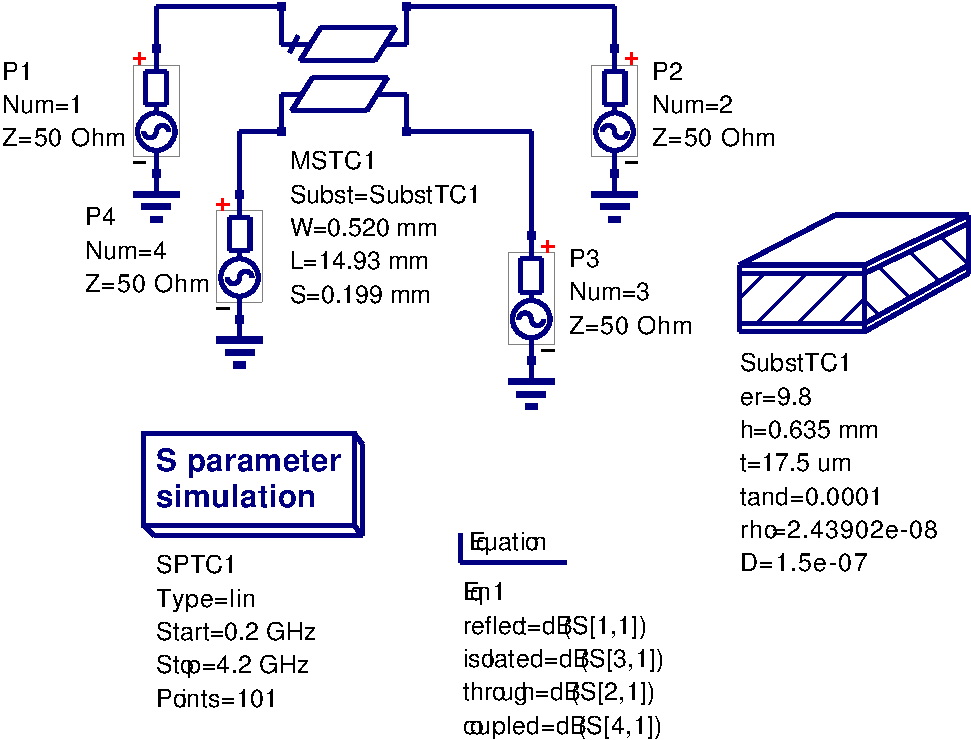
\includegraphics[width=0.8\linewidth]{mscouplersch}
  \caption{final microstrip coupler schematic}
  \label{fig:mscouplersch}
\end{figure}
\FloatBarrier

Now select \textbf{Simulation} $\rightarrow$ \textbf{Simulate} from
the menubar or just press \textbf{F2} to simulate the schematic.

\addvspace{12pt}

When the simulation windows disappears then choose a
\textbf{Cartesian} diagram from the left hand selection view and place
the diagram into the (yet empty) data display area.  Double click the
\textbf{through}, \textbf{reflect}, \textbf{isolated} and
\textbf{coupled} data items in order to add it to the diagram within
the diagram dialog as shown in figure \ref{fig:diagramdialog}.

\begin{figure}[ht]
  \centering
  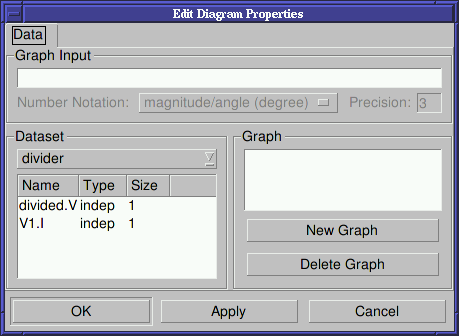
\includegraphics[width=0.6\linewidth]{diagramdialog}
  \caption{diagram dialog}
  \label{fig:diagramdialog}
\end{figure}
\FloatBarrier

Press \textbf{OK} to finish the diagram dialog.  Afterwards you will
see the following diagram.

\begin{figure}[ht]
  \centering
  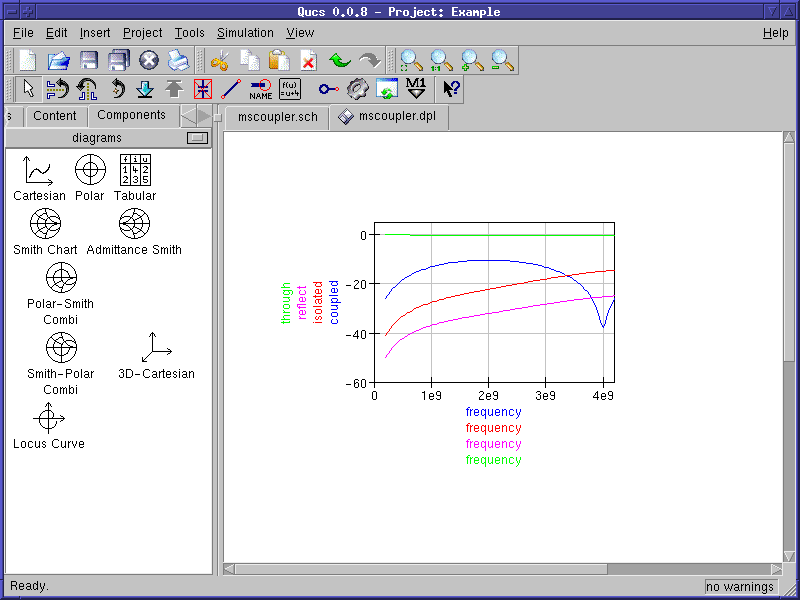
\includegraphics[width=1\linewidth]{coupleddpl}
  \caption{microstrip coupler simulation results}
  \label{fig:coupleddpl}
\end{figure}
\FloatBarrier

\tutsubsection{Suggested improvements}

By use of the diagram dialog (double click the diagram) you may
improve\footnote{... to feel even better.} the data visualization as
you see it fit.  I manually fixed the y-axis limits, set markers and
set curve thickness to 2 points.  Also I entered a common x-axis
label.  See figure \ref{fig:mscouplerdpl} how it looks now.

\begin{figure}[ht]
  \centering
  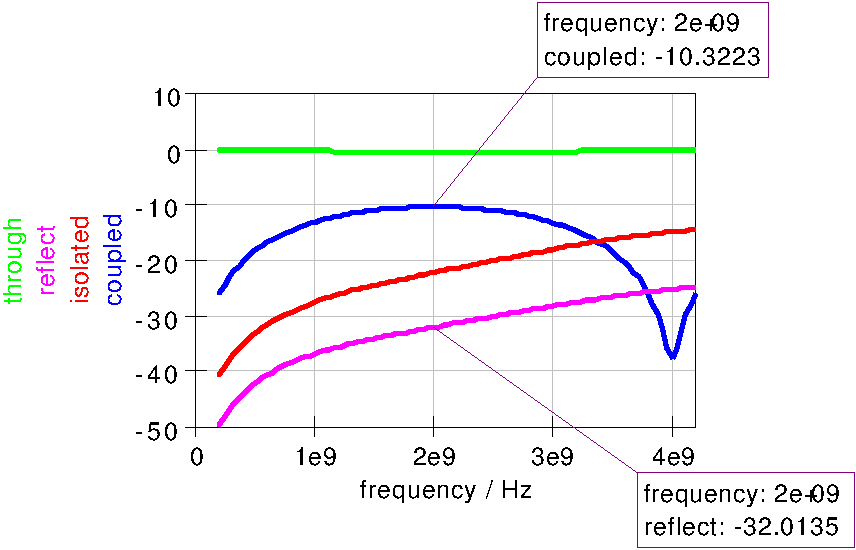
\includegraphics[width=0.8\linewidth]{mscouplerdpl}
  \caption{directional coupler simulation result diagram}
  \label{fig:mscouplerdpl}
\end{figure}
\FloatBarrier

The marker on the \textbf{coupled} curve shows a coupling factor of
\textbf{-10.32} at a frequency of 2GHz (double click marker to change
precision of the marker data).  This is a bit way off for which we
tried to design it for.

\addvspace{12pt}

Seems like coupling between the lines is a bit too weak.  So we reduce
the gap between the strip conductors \textbf{S} by $16.5\micro\meter$ to
be \textbf{0.1825 mm} and simulate again.

\begin{figure}[ht]
  \centering
  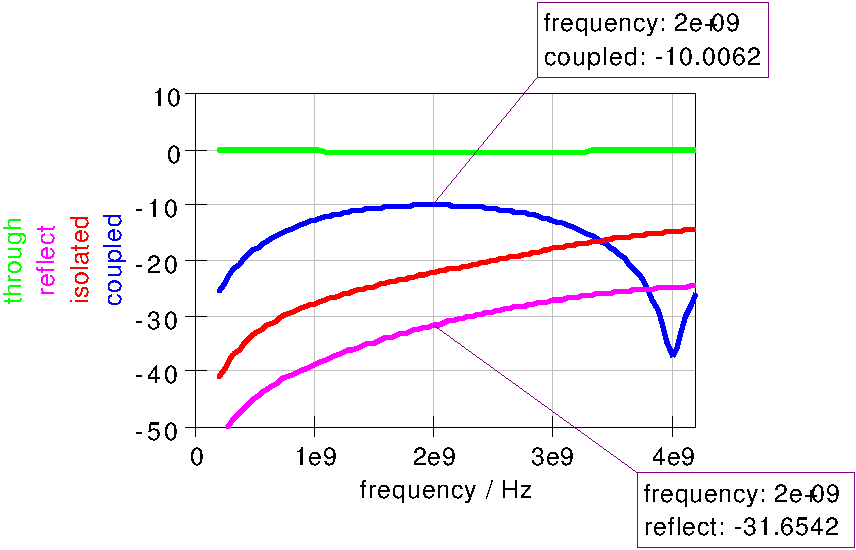
\includegraphics[width=0.8\linewidth]{mscouplerdpl_opt}
  \caption{optimized directional coupler simulation result diagram}
  \label{fig:mscouplerdpl_opt}
\end{figure}
\FloatBarrier

Finally a perfect\footnote{... to feel great.} 10dB coupling as shown
in figure \ref{fig:mscouplerdpl_opt}.

\tutsubsection{Remaining thinkabouts}

The diagram in figure \ref{fig:mscouplerdpl_opt} shows a reflection
coefficient of about -31.7dB.  The isolation (about -22.2dB) is not as
good as planned as well.  So -- what happened with my design
equations?

\addvspace{12pt}

Have a look at figure \ref{fig:trcalc}.  In the \textbf{Calculated
Results} panel you see \textbf{ErEff Even} and \textbf{ErEff Odd}
differing significantly which is not what we expect from an ideal
backward coupler:
\begin{equation*}
\varepsilon_{r,eff,e} = \varepsilon_{r,eff,o}
\end{equation*}
This ``problem'' arises from the fact that there are two dieletrica
involved: air and the substrate.  Part of the electromagnetic fields
cross air and part of them the substrate.  You can inhibit this by a
dielectric overlay.  It's more expensive to produce but improves your
results.
